\documentclass{beamer}

\mode<presentation> {

% The Beamer class comes with a number of default slide themes
% which change the colors and layouts of slides. Below this is a list
% of all the themes, uncomment each in turn to see what they look like.

%\usetheme{default}
%\usetheme{AnnArbor}
%\usetheme{Antibes}
%\usetheme{Bergen}
%\usetheme{Berkeley}
%\usetheme{Berlin}
%\usetheme{Boadilla}
%\usetheme{CambridgeUS}
%\usetheme{Copenhagen}
%\usetheme{Darmstadt}
\usetheme{Dresden}
%\usetheme{Frankfurt}
%\usetheme{Goettingen}
%\usetheme{Hannover}
%\usetheme{Ilmenau}
%\usetheme{JuanLesPins}
%\usetheme{Luebeck}
%\usetheme{Madrid}
%\usetheme{Malmoe}
%\usetheme{Marburg}
%\usetheme{Montpellier}
%\usetheme{PaloAlto}
%\usetheme{Pittsburgh}
%\usetheme{Rochester}
%\usetheme{Singapore}
%\usetheme{Szeged}
%\usetheme{Warsaw}

% As well as themes, the Beamer class has a number of color themes
% for any slide theme. Uncomment each of these in turn to see how it
% changes the colors of your current slide theme.

%\usecolortheme{albatross}
%\usecolortheme{beaver}
%\usecolortheme{beetle}
%\usecolortheme{crane}
%\usecolortheme{dolphin}
%\usecolortheme{dove}
%\usecolortheme{fly}
%\usecolortheme{lily}
%\usecolortheme{orchid}
%\usecolortheme{rose}
%\usecolortheme{seagull}
%\usecolortheme{seahorse}
\usecolortheme{whale}
%\usecolortheme{wolverine}

%\setbeamertemplate{footline} % To remove the footer line in all slides uncomment this line
%\setbeamertemplate{footline}[page number] % To replace the footer line in all slides with a simple slide count uncomment this line

%\setbeamertemplate{navigation symbols}{} % To remove the navigation symbols from the bottom of all slides uncomment this line
}

\usepackage{graphicx} % Allows including images
\usepackage{booktabs} % Allows the use of \toprule, \midrule and \bottomrule in tables
\usepackage[backend=bibtex,natbib=true,sorting=none,style=nature]{biblatex}
\bibliography{../MT.bib}

%----------------------------------------------------------------------------------------
%	TITLE PAGE
%----------------------------------------------------------------------------------------

\title[Ultrafast manipulation of antiferromagnetic insulators]{Ultrafast manipulation of Heisenberg exchange and Dzyaloshinskii Moriya interactions in antiferromagnetic insulators} % The short title appears at the bottom of every slide, the full title is only on the title page

%\author{Juan Manuel Losada Sosnovsky} % Your name
%\autoref{asdf}{asdf}
%\author[author1]{author1\inst{1}\\[1ex]  {\small supervisor1\inst{1,2}}}
\author[Juan Manuel Losada Sosnovsky]{Juan Manuel Losada Sosnovsky\\[10mm]{\small Supervisor: Alireza Qaiumzadeh}}
\institute[NTNU] % Your institution as it will appear on the bottom of every slide, may be shorthand to save space
{
QuSpin (NTNU)
}
\date{\today} % Date, can be changed to a custom date
\newcommand{\bs}[1] {\boldsymbol{#1}}
\begin{document}

\begin{frame}
\titlepage % Print the title page as the first slide
\end{frame}

%----------------------------------------------------------------------------------------
%	PRESENTATION SLIDES
%----------------------------------------------------------------------------------------

%------------------------------------------------
\section{First Section} % Sections can be created in order to organize your presentation into discrete blocks, all sections and subsections are automatically printed in the table of contents as an overview of the talk
%------------------------------------------------

\subsection{Subsection Example} % A subsection can be created just before a set of slides with a common theme to further break down your presentation into chunks

\begin{frame}
\frametitle{Spintronics}
Study and use the intrinsic spin of the electrons, in addition to their charge, to build devices. Example: Magnetoresistive random access memory.

%\begin{figure}
%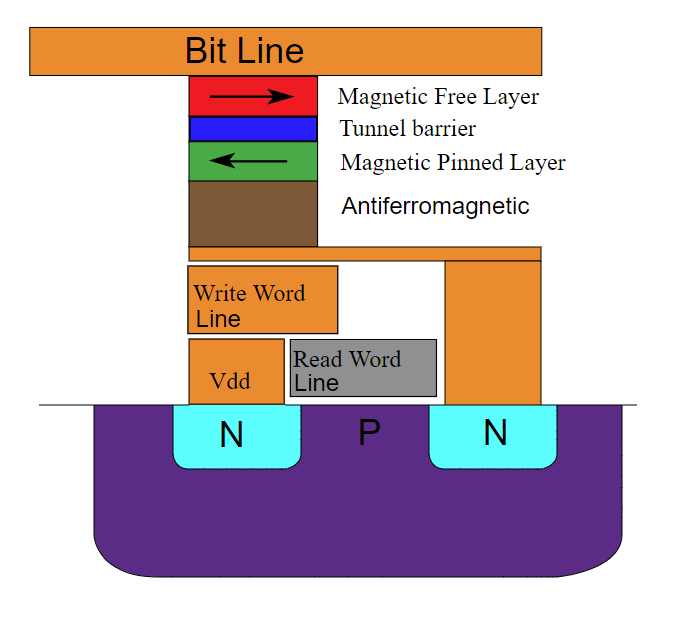
\includegraphics[width=0.5\linewidth]{../Figures/fm_device.png}
%\caption{Source: Wikipedia}
%\end{figure}

\begin{figure}
  \begin{minipage}[c]{0.6\textwidth}
    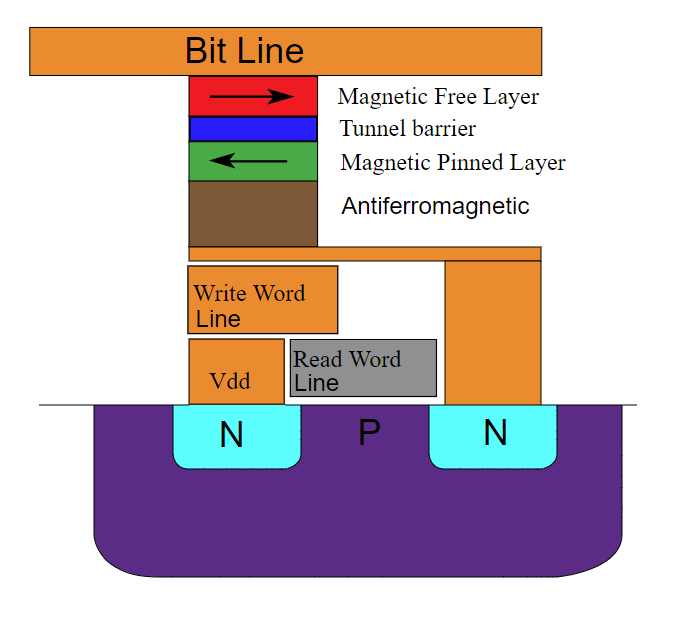
\includegraphics[width=\textwidth]{../Figures/fm_device.png}
  \end{minipage}\hfill
  \begin{minipage}[c]{0.2\textwidth}
    \caption{Source: Wikipedia} \label{fig:1}
  \end{minipage}
\end{figure}

\end{frame}

%------------------------------------------------

\begin{frame}
\frametitle{Antiferromagnetic Spintronics}
The development of information technology demands devices with high storage density, high energy efficiency and high write-read speeds. Antiferromagnets have appear as a natural alternative to ferromagnets due to some advantages: 
\begin{itemize}
\item Robustness against magnetic disturbances.
\item No hysteresis loss.
\item Produce no stray fields.
\item Ultrafast dynamics (femtosecond).
\end{itemize}
\end{frame}

\begin{frame}
\frametitle{Antiferromagnetic Spintronics}

\begin{figure}
  \begin{minipage}[c]{0.6\textwidth}
    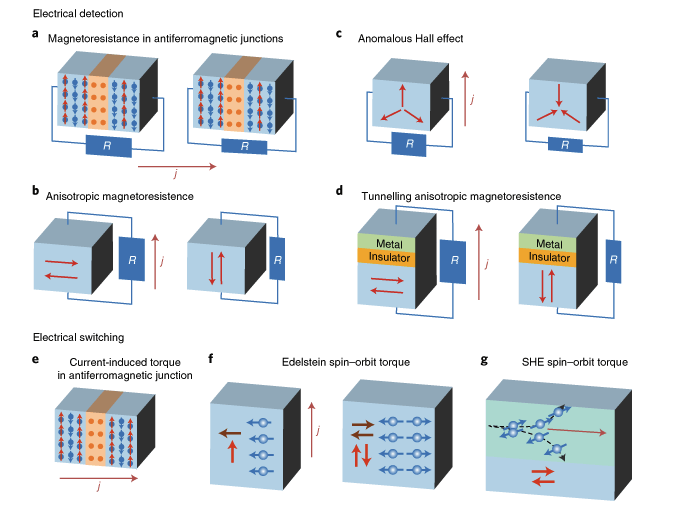
\includegraphics[width=\textwidth]{../Figures/afm_device.png}
  \end{minipage}\hfill
  \begin{minipage}[c]{0.2\textwidth}
    \caption{Source: Nature, Spin transport and spin torque in antiferromagnetic devices} \label{fig:2}
  \end{minipage}
\end{figure}

\end{frame}

%------------------------------------------------

\begin{frame}
\frametitle{Manipulation of the spin state}
\begin{block}{Heisenberg model}
\begin{equation} 
\hat{H} = \sum_{\langle i,j \rangle} J \boldsymbol{S}_i \boldsymbol{S}_j \nonumber
\end{equation}
In antiferromagnets $J > 0$ ($J < 0$ for ferromagnets). Mentink, J. H. et al. showed that it is possible to manipulate the exchange constant by applying a laser field. $J = J_0 + \Delta J$.
\end{block}
\end{frame}

%------------------------------------------------

\begin{frame}
\frametitle{Manipulation of the spin state}
\begin{block}{Heisenberg model with DMI}
\begin{equation} 
\hat{H} = \sum_{\langle i,j \rangle} J \boldsymbol{S}_i \boldsymbol{S}_j + \sum_{\langle i,j \rangle} \vec{D}_{ij}\boldsymbol{S}_i \times \boldsymbol{S}_j\nonumber
\end{equation}

Under some circumstances this Hamiltonian describes a canted antiferromagnet.

\begin{figure}
  \begin{minipage}[c]{0.6\textwidth}
    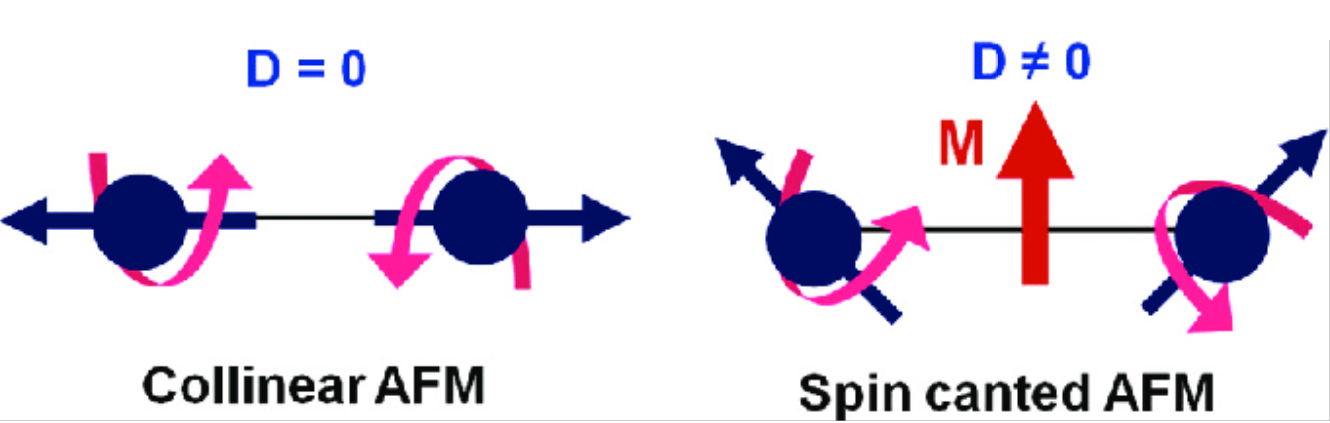
\includegraphics[width=\textwidth]{../Figures/dmi_canting.png}
  \end{minipage}\hfill
  \begin{minipage}[c]{0.2\textwidth}
    \caption{Source: Nanoscale} \label{fig:3}
  \end{minipage}
\end{figure}

\end{block}
\end{frame}

\begin{frame}
\frametitle{Manipulation of the spin state}
If we can manipulate $J$ and $D$ we can control the canting angle.
\begin{figure}
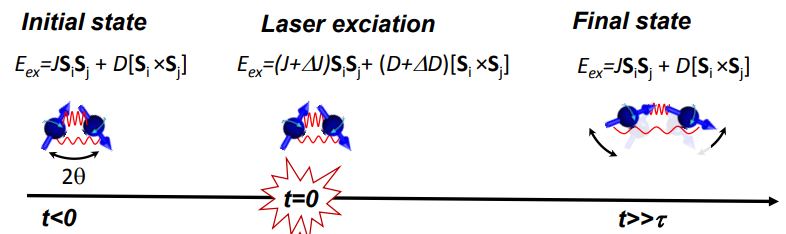
\includegraphics[width=1\linewidth]{../Figures/canted_afm.png}
\caption{Source: Kimmel presentation}
\end{figure}
\end{frame}

\begin{frame}
\frametitle{Manipulation of the spin state}
We need $\frac{J}{D} \neq \frac{J+\Delta J}{D+\Delta D}$.
\\[10mm]
However, $\frac{J}{D} = \frac{J+\Delta J}{D+\Delta D}$.
\end{frame}

\begin{frame}
\frametitle{Manipulation of the spin state}
\begin{block}{Kane-Mele-Hubbard model}
\begin{equation}
\hat{H}_{\text{KMH}} = -t_1\sum_{\langle i j \rangle \sigma} \hat{c}^{\dagger}_{i\sigma}\hat{c}_{j\sigma} + i\Delta \sum_{\langle \langle i j \rangle \rangle \sigma \sigma'} \hat{c}^{\dagger}_{i\sigma} \nu_{ij} \sigma^z_{\sigma \sigma'} \hat{c}_{j\sigma'} + \text{U}\hat{D}\nonumber
\end{equation}

It leads to a spin Hamiltonian:

\begin{equation}
\hat{H}_{\text{KMH}}^{\text{eff}} = \sum_{\langle i,j \rangle} J_{ij} \bs{S}_i \bs{S}_j + \sum_{\langle \langle i,j \rangle \rangle} \bs{S}_i \bs{\Gamma}_{ij} \bs{S}_j \nonumber
\end{equation}

\end{block}
\end{frame}

\begin{frame}
\frametitle{Manipulation of the spin state}
\begin{block}{Modified Kane-Mele-Hubbard model}
\begin{equation}
\hat{H} = - t_1\sum_{\langle i,j \rangle, \sigma} \hat{c}_{i \sigma}^\dagger \hat{c}_{j \sigma} + 
	\sum_{\langle \langle i,j \rangle \rangle, \sigma}(t_2 + i\Delta\nu_{ij}\sigma^z_{\sigma, \sigma})\hat{c}_{i \sigma}^\dagger \hat{c}_{j \sigma} + 
	\text{U}\hat{D}\nonumber
\end{equation}

It leads to a spin Hamiltonian:

\begin{equation}
\hat{H}_{\text{eff}}(t) = \sum_{\langle i,j \rangle} J_{1,ij}\bs{S}_i\bs{S}_j + \sum_{\langle \langle i,j \rangle \rangle} \left\{ J_{2,ij}\bs{S}_i\bs{S}_j + \bs{D}_{2,ij} \bs{S}_i \times \bs{S}_j + \bs{S}_i \bs{\Gamma}_{ij} \bs{S}_j \right\} \nonumber
\end{equation}

What we wanted, in this case if we apply light $\frac{J}{D} \neq \frac{J+\Delta J}{D + \Delta D}$.

\end{block}
\end{frame}

\begin{frame}
\begin{figure}
  \begin{minipage}[c]{0.5\textwidth}
    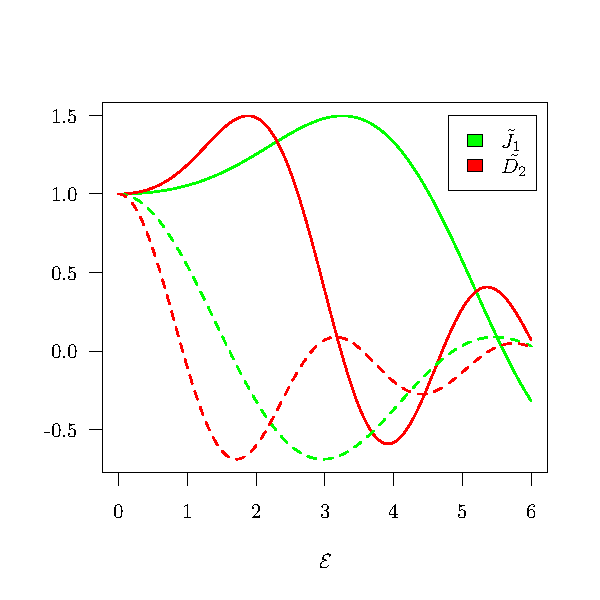
\includegraphics[width=\textwidth]{../Figures/NNvsNNN1.pdf}
  \end{minipage}\hfill
  \begin{minipage}[c]{0.5\textwidth}
    \caption{$\frac{J_{1}}{J_{1}^0}$ and $\frac{D_{2,ij}}{D_{2,ij}^0}$ are plotted as function of $\mathcal{E}$. Similar results are obtained in \cite{Mentink2015} for $J_{1}$. Solid lines are for $\omega = 4$ and dashed lines are for $\omega = 14$.}
  \end{minipage}
\end{figure}
\footfullcite{Mentink2015}
\end{frame}

\begin{frame}
\Huge{\centerline{The End}}
\end{frame}

\end{document}